\documentclass[twoside]{article}
\setlength{\oddsidemargin}{0 in}
\setlength{\evensidemargin}{0 in}
\setlength{\topmargin}{-0.6 in}
\setlength{\textwidth}{6.5 in}
\setlength{\textheight}{8.5 in}
\setlength{\headsep}{0.75 in}
\setlength{\parindent}{0 in}
\setlength{\parskip}{0.1 in}

\usepackage{url}
\usepackage{titlesec}
\setcounter{secnumdepth}{3}
\usepackage{palatino}
\usepackage{marginnote}
\usepackage{multirow}
\usepackage{easybmat,bigdelim,arydshln}
\usepackage[authoryear,round]{natbib}
\usepackage{amssymb,amsmath,amsthm,amsfonts}
\usepackage{mathtools}
%\usepackage{nicematrix}
\usepackage{arydshln}
\usepackage{caption}
\usepackage{hyperref}
\usepackage{tcolorbox}
\tcbuselibrary{skins, breakable, theorems}
\usepackage{newpxtext,newpxmath}
\usepackage{longtable}
\usepackage{enumitem}
\makeatletter

\let\bar\overline

\setlist[itemize]{topsep=0pt,leftmargin=10pt,itemsep=-0.2em}
\usepackage{xcolor}
\usepackage{tikz}
\usepackage{pgfplots}
\pgfplotsset{compat = newest}
\usetikzlibrary{patterns,decorations.pathreplacing,decorations.markings,fit,shapes.geometric,angles,quotes,arrows}
\usepgfplotslibrary{fillbetween}

\usepackage{ifthen}
\usepackage{tikz-3dplot}

\pgfdeclarelayer{ft}
\pgfdeclarelayer{bg}
\pgfsetlayers{bg,main,ft}

\hypersetup{
    colorlinks,
    citecolor=red,
    filecolor=black,
    linkcolor=violet,
    urlcolor=blue
}

\definecolor{myblue}{cmyk}{1,.72,0,.38}
\definecolor{mypurple}{cmyk}{.57,1,0,.58}
\definecolor{myred}{cmyk}{0,.88,.88,.58}
\definecolor{mygreen}{cmyk}{1,0,.69,.66}
\definecolor{myorange}{cmyk}{0,.58,100,.20}
\definecolor{glaucous}{rgb}{0.38, 0.51, 0.71}

\makeatletter
\renewcommand{\thefigure}{\thesection.\arabic{figure}}
\newtheoremstyle{indented}
  {3pt}% space before
  {3pt}% space after
  {\addtolength{\@totalleftmargin}{3.5em}
   \addtolength{\linewidth}{-3.5em}
   \parshape 1 3.5em \linewidth}% body font
  {}% indent
  {\bfseries}% header font
  {.}% punctuation
  {.5em}% after theorem header
  {}% header specification (empty for default)
\makeatother

\newcommand{\ind}{\perp\!\!\!\perp}

\theoremstyle{definition}
\newtheorem{defin}{Definition}[section] % Creates a new counter, number within section
\newtheorem{prt}[defin]{Remark} 
\newtheorem{prts}[defin]{Remarks} % Again share defin's counter
\newtheorem{exmp}[defin]{Example} % etc.
\newtheorem{exmps}[defin]{Examples}
\newtheorem*{note}{Note}
\tcbuselibrary{theorems}

% use counter*=defin to make each tcbtheorem share defin's counter

\newtcbtheorem[use counter*=defin, number within=section]{definition}{Definition}{enhanced, breakable,
    colback = white, colframe = red!55!black, colbacktitle = red!55!black, attach boxed title to top left = {yshift = -2.5mm, xshift = 3mm}, boxed title style = {sharp corners},fonttitle=\bfseries}{def}

\newtcbtheorem[use counter*=defin, number within=section]{theorem}{Theorem}{enhanced, breakable,
    colback = white, colframe = blue!45!black, colbacktitle = blue!45!black, attach boxed title to top left = {yshift = -2.5mm, xshift = 3mm}, boxed title style = {sharp corners},fonttitle=\bfseries}{thm}
    
\newtcbtheorem[use counter*=defin, number within=section]{proposition}{Proposition}{enhanced, breakable,
    colback = white, colframe = teal, colbacktitle = teal, attach boxed title to top left = {yshift = -2.5mm, xshift = 3mm}, boxed title style = {sharp corners},fonttitle=\bfseries}{prop}

\newtcbtheorem[use counter*=defin, number within=section]{lemma}{Lemma}{enhanced, breakable,
    colback = white, colframe = orange!80!black, colbacktitle = orange!80!black, attach boxed title to top left = {yshift = -2.5mm, xshift = 3mm}, boxed title style = {sharp corners},fonttitle=\bfseries}{lemma}

\newtcbtheorem[use counter*=defin, number within=section]{example}{Example}{enhanced, breakable,
    colback = white, colframe = yellow!60!black, colbacktitle = yellow!60!black, attach boxed title to top left = {yshift = -2.5mm, xshift = 3mm}, boxed title style = {sharp corners},fonttitle=\bfseries}{exmp}

\newtcbtheorem[use counter*=defin, number within=section]{assumption}{Assumption}{enhanced, breakable,
    colback = white, colframe = violet!60!white, colbacktitle = violet!60!white, attach boxed title to top left = {yshift = -2.5mm, xshift = 3mm}, boxed title style = {sharp corners},fonttitle=\bfseries}{assump}

\newtcbtheorem[use counter*=defin, number within=section]{algorithm}{Algorithm}{enhanced, breakable,
    colback = white, colframe = green!55!black, colbacktitle = green!55!black, attach boxed title to top left = {yshift = -2.5mm, xshift = 3mm}, boxed title style = {sharp corners},fonttitle=\bfseries}{algm}
%\newtcolorbox{example}[1]{enhanced, breakable, colback = white, colframe = orange!85!black, colbacktitle = orange!85!black, attach boxed title to top left = {yshift = -2.5mm, xshift = 3mm}, boxed title style = {sharp corners},fonttitle=\bfseries, title={Example: #1}}

\newtcbox{\myhl}[1][white]
  {on line, arc = 0pt, outer arc = 0pt,
    colback = #1!20!white, colframe = #1!50!black,
    boxsep = 0pt, left = 1pt, right = 1pt, top = 1pt, bottom = 1pt, boxrule = 0pt, bottomrule =0pt, toprule =0pt}
    
\newtcbox{\myhlrule}[1][white]
  {on line, arc = 0pt, outer arc = 0pt,
    colback = #1!20!white, colframe = #1!50!black,
    boxsep = 0pt, left = 1pt, right = 1pt, top = 1pt, bottom = 1pt, boxrule = 0pt, bottomrule =0.5pt, toprule =0.5pt}
%
% The following commands set up the lecnum (lecture number)
% counter and make various numbering schemes work relative
% to the lecture number.
%
\newcounter{lecnum}
\renewcommand{\thepage}{\thelecnum-\arabic{page}}
\renewcommand{\thesection}{\thelecnum.\arabic{section}}
\renewcommand{\theequation}{\thelecnum.\arabic{equation}}
\renewcommand{\thefigure}{\thelecnum.\arabic{figure}}
\renewcommand{\thetable}{\thelecnum.\arabic{table}}

\newcommand{\sidenotes}[1]{\marginnote{\raggedright\scriptsize#1}}
%
% The following macro is used to generate the header.
%
\newcommand{\lecture}[6]{
   \pagestyle{myheadings}
   \thispagestyle{plain}
   \newpage
   \setcounter{lecnum}{#1}
   \setcounter{page}{1}
   \noindent
   \begin{center}
   \framebox{
      \vbox{\vspace{2mm}
    \hbox to 6.28in { {\bf Econometrics
	\hfill \today} }
       \vspace{4mm}
       \hbox to 6.28in { {\Large \hfill Topic #1: #2  \hfill} }
       \vspace{2mm}
       \hbox to 6.28in { {\it #3 \hfill by #4} }
      \vspace{2mm}}
   }
   \end{center}
   \markboth{Week #1: #2}{Week #1: #2}

   {\bf Key points}: {#5}

   {\bf Disclaimer}: {\it #6}
   \vspace*{4mm}
}
%

\tikzset{-stealth-/.style={decoration={
  markings,
  mark=at position #1 with {\arrow{stealth}}},postaction={decorate}}}

  \tikzset{tangent/.style={
    decoration={
        markings,% switch on markings
        mark=
            at position #1
            with
            {
                \coordinate (tangent point-\pgfkeysvalueof{/pgf/decoration/mark info/sequence number}) at (0pt,0pt);
                \coordinate (tangent unit vector-\pgfkeysvalueof{/pgf/decoration/mark info/sequence number}) at (1,0pt);
                \coordinate (tangent orthogonal unit vector-\pgfkeysvalueof{/pgf/decoration/mark info/sequence number}) at (0pt,1);
            }
    },
    postaction=decorate
},
use tangent/.style={
    shift=(tangent point-#1),
    x=(tangent unit vector-#1),
    y=(tangent orthogonal unit vector-#1)
},
use tangent/.default=1}

\tikzstyle{terminator} = [rectangle, draw, thick, text centered, rounded corners, minimum height=2em]
\tikzstyle{process} = [rectangle, draw, thick, text centered, minimum height=2em]
\tikzstyle{decision} = [diamond, draw, thick, text centered, minimum width=3cm, minimum height=0.5cm]
\tikzstyle{data}=[trapezium, draw, thick, text centered, trapezium left angle=60, trapezium right angle=120, minimum height=2em]
\tikzstyle{arrow} = [thick,->,>=stealth]

\begin{document}
\lecture{17}{False Discovery Rate (FDR) and Knockoffs}{}{Sai Zhang}{Constructing knockoff variables to control FDR when estimating regression coefficients.}{The note is built on Prof. \hyperlink{http://faculty.marshall.usc.edu/jinchi-lv/}{Jinchi Lv}'s lectures of the course at USC, DSO 607, High-Dimensional Statistics and Big Data Problems.}
%\footnotetext{These notes are partially based on those of Nigel Mansell.}

\section{Motivation}
Consider the classical linear regression setting
$$
\mathbf{y} = \mathbf{X}\boldsymbol{\beta} + \boldsymbol{\epsilon}
$$
where $\boldsymbol{\beta}\in\mathbb{R}^p$ is the unknown vector of coefficients and $\boldsymbol{\epsilon}\sim \mathcal{N}(\mathbf{0},\sigma^2\mathbf{I})$. In a high-dimensional problem, we would like to just select a subset of all variables $\hat{S}\subset \left\{ 1,\cdots,p \right\}$ s.t. conditional on $\left\{\mathbf{X}_j\right\}_{j\in\hat{S}}$, $\mathbf{y}$ is \textbf{independent} of all other variables, we can define the \myhl[myblue]{\textbf{False Discovery Rate}} \textbf{(FDR)} in can be defined as 
\begin{definition}{False Discovery Rate (FDR)}{FDR}
    \begin{align*}
        \mathrm{FDR} = \mathbb{E}(\mathrm{FDP}) = \mathbb{E}\left[ \frac{\lvert \hat{\mathcal{S}}\cap \mathcal{H}_0 \rvert}{ \lvert \hat{\mathcal{S}} \rvert } \textcolor{myred}{ =\frac{\#\left\{ j:j\in\hat{\mathcal{S}}\setminus \mathcal{S}\right\} }{\#\left\{ j:j\in\hat{\mathcal{S}}\right\} }} \right]
    \end{align*}
    where $\mathcal{H}_0\subset \left\{1,\cdots,p\right\}$ is the set of \myhl[myred]{\textbf{{null}}} variables: $\mathbf{X}_j$ is {\textbf{null}} iff $\mathbf{Y}$ is independent of $\mathbf{X}_j$ conditional on the other variables $\mathbf{X}_{-j}=\left\{\mathbf{X}_1,\cdots,\mathbf{X}_p\right\}\setminus \left\{\mathbf{X}_j\right\}$.
\end{definition}

In this note, we consider a series of knockoff-based methods to control FDR. They all follow a common procedure:
\begin{itemize}
    \item \textbf{\underline{Step 1}}: Construct Knockoffs 
    \item \textbf{\underline{Step 2}}: Calculate test statistics for both original and knockoff variables
    \item \textbf{\underline{Step 3}}: Calculate a threshold for the test statistics, controling for a desired FDR level
    \item \textbf{\underline{Step 4}}: Select variables that pass the threshold
\end{itemize}

\section{Barber and Candes (2015)}
\paragraph{Constructing the knockoffs}
\citet{Barber2015} construct the knockoffs by the following procedure
\begin{itemize}
    \item Calculate the Gram matrix $\boldsymbol{\Sigma}=\mathbf{X'X}$ for the normalized original variables, where $\Sigma_{jj}=\left\Vert \mathbf{X}_j \right\Vert^2_2 = 1$
    \item Construct the knockoffs $\tilde{\mathbf{X}}$ s.t. 
    \begin{align*}
        \tilde{\mathbf{X}}'\tilde{\mathbf{X}} &= \boldsymbol{\Sigma} & {\mathbf{X}}'\tilde{\mathbf{X}} = \boldsymbol{\Sigma} -\mathrm{diag}\left\{\mathbf{s}\right\}
    \end{align*}
    where $\mathbf{s}\in\mathbb{R}^p_{+}$ is a p-dimensional non-negative vector (larger $s_j$ indicates higher power) and
    \begin{itemize}
        \item $\tilde{\mathbf{X}}$ exhibits the \myhl[myblue]{\textbf{same}} covariance structrue as the original design $\mathbf{X}$
        \item The correlation between distinct original variables and knockoffs are the same as between the originals: $$ \mathbf{X}_j'\tilde{\mathbf{X}}_k = \mathbf{X}_j'{\mathbf{X}}_k,\ \forall j\neq k $$
        \item The correlation between the original variables and their own knockoffs is \myhl[myblue]{\textbf{less than 1}} $$ \mathbf{X}_j'\tilde{\mathbf{X}}_j = \Sigma_{jj}-s_j = 1-s_j $$
    \end{itemize}
    To construct such knockoffs, 
    \begin{itemize}
        \item Given a proper $\mathbf{s}$, if $n \geq  2p$, then  $$ \tilde{\mathbf{X}} = \mathbf{X}(\mathbf{I}-\boldsymbol{\Sigma}^{-1}\mathrm{diag}\left\{\mathbf{s}\right\}) + \tilde{\mathbf{U}}\mathbf{C} $$ where $\tilde{\mathbf{U}}\in \mathbb{R}^{n\times p}$ is an \myhl[myblue]{\textbf{orthonormal}} matrix s.t. $\tilde{\mathbf{U}}'\mathbf{X}=\mathbf{0}$ and $\mathbf{C'C}=2\mathrm{diag}\left\{\mathbf{s}\right\} - \mathrm{diag}\left\{\mathbf{s}\right\}\boldsymbol{\Sigma}^{-1}\mathrm{diag}\left\{\mathbf{s}\right\} \geq \mathbf{0}$
        \item A sufficient and necessary condition for $\tilde{\mathbf{X}}$ to exist: $\mathrm{diag}\left\{\mathbf{s}\right\} \leq 2\boldsymbol{\Sigma}$
    \end{itemize}
    2 types of knockoffs can be constructed, following these procedures
    \begin{itemize}
        \item[T1] \underline{\textbf{Equi-correlated}} knockoffs: set $s_j=2\lambda_{\min}(\boldsymbol{\Sigma}) \wedge 1$ for all $j$, then $\langle \mathbf{X}_j,\tilde{\mathbf{X}}_j \rangle = 1-2\lambda_{\min}(\boldsymbol{\Sigma}) \wedge 1$ for all $j$. This is essentially minimizing $\left\vert \langle \mathbf{X}_j,\tilde{\mathbf{X}}_j \rangle \right\vert$ 
        \item[T2] \underline{\textbf{SDP}} knockoffs: solve the convex problem \begin{align*}
            \arg\min_{\mathbf{x}} \sum_j (1-s_j) & & s.t. 0 \leq s_j \leq 1, \mathrm{diag}\left\{ \mathbf{s}\right\}\leq 2\boldsymbol{\Sigma}
        \end{align*}
        which is essentially minimizing the average of $ \langle \mathbf{X}_j,\tilde{\mathbf{X}}_j \rangle $ 
    \end{itemize}
\end{itemize}

\paragraph{Calculate test statistics} Define and calculate test statistics $W_j$ for each $\beta_j\in\left\{ 1,\cdots,p \right\}$ using $\begin{bmatrix} \mathbf{X} & \tilde{\mathbf{X}} \end{bmatrix}$:
\begin{itemize}
    \item the test statistic $W_j$ should be constructed s.t. large positive values are evidence against the null hypothesis $\beta_j =0$, for example, consider a Lasso on $\begin{bmatrix} \mathbf{X} & \tilde{\mathbf{X}} \end{bmatrix}$ $$ \hat{\beta}(\lambda) = \arg\min_{\mathbf{b}}\left\{ \frac{1}{2}\left\Vert \mathbf{y}-\begin{bmatrix} \mathbf{X} & \tilde{\mathbf{X}} \end{bmatrix} \mathbf{b} \right\Vert^2_2 + \lambda\left\Vert \mathbf{b} \right\Vert \right\} _1 $$ where $\lambda$ is the point on the Lasso path at which the feature enters the model as $$ Z_j = \sup \left\{ \lambda: \hat{\beta}_j(\lambda)\neq 0 \right\} $$ and set $W_j = (Z_j \vee \tilde{Z}_j)\cdot \begin{cases} +1, &Z_j>\tilde{Z}_j \\ -1, & Z_j<\tilde{Z}_j \end{cases}$\footnote{Other choices of $W_j$ are $W_j =\left\vert\mathbf{X}'_j\mathbf{y} \right\vert - \left\vert\tilde{\mathbf{X}}'_j\mathbf{y} \right\vert $, or $\left\vert \hat{\beta}^{\mathrm{LS}}_j \right\vert-\left\vert \hat{\beta}^{\mathrm{LS}}_{j+p} \right\vert$} 
    \item In general, the statistics $W$ should satisfy the \myhl[myblue]{\textbf{sufficient}} property and \myhl[myblue]{\textbf{anti-symmetry}} property:
    \begin{definition}{Property of Test Statistics $W_j$}{statistic_property}
        The test statistic $W_j$ is said to obey
        \begin{itemize}
            \item the \myhl[myred]{\textbf{sufficient}} property if $\mathbf{W}$ depends \underline{\textit{only}} on the Gram matrix and on feature-response inner products, that is $$ \mathbf{W} = f\left( \begin{bmatrix} \mathbf{X} & \tilde{\mathbf{X}} \end{bmatrix}'\begin{bmatrix} \mathbf{X} & \tilde{\mathbf{X}} \end{bmatrix},\begin{bmatrix} \mathbf{X} & \tilde{\mathbf{X}} \end{bmatrix}'\mathbf{y} \right) $$
            \item the \myhl[myred]{\textbf{antisymmetry}} property if swapping the original $\mathbf{X}_j$ and its knockoff $\tilde{\mathbf{X}}_j$ has the effect of \textbf{switching the sign} of $W_j$, that is $$ W_j(Z_j,\tilde{Z}_j)= -W_j (\tilde{Z}_j,Z_j) $$
        \end{itemize}
    \end{definition}
\end{itemize}

\paragraph*{Calculate a threshold for the test statistics} After defining the test statistic, we then
\begin{itemize}
    \item Let $q$ be the target FDR, define the data-dependent threshold $T$ as $$ T =\min\left\{ t\in\mathcal{W}: \frac{\# \left\{j:W_j\leq -t \right\}}{\# \left\{j:W_j\geq t \right\} \vee 1} \leq  q \right\} $$ where $\mathcal{W}=\left\{ \left\vert W_j \right\vert: j=1,\cdots,p \right\} \setminus \left\{ 0 \right\}$ is the set of unique non-zero values attained by $\lvert W_j \rvert$'s.
    \begin{figure}[ht]
        \centering
        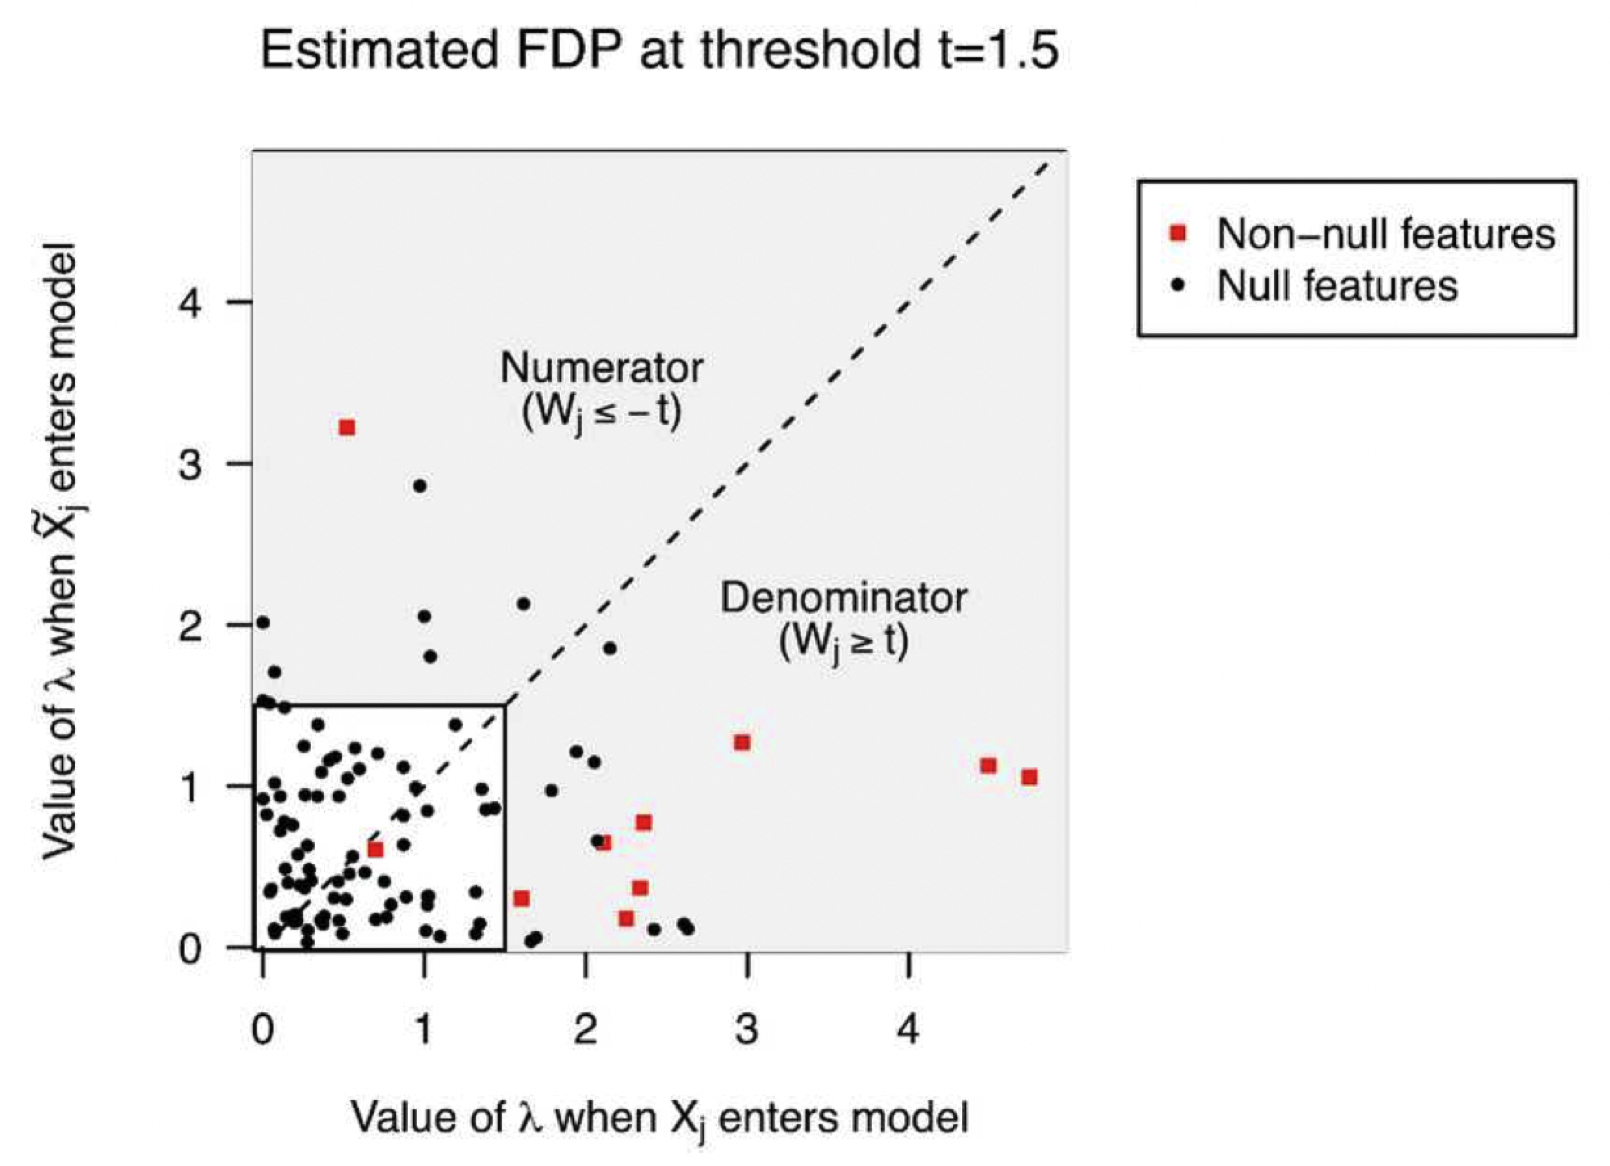
\includegraphics[width = 0.6 \textwidth]{figures/note17_visualizingFDR.png}
        \caption{Visualizing Test Statistic Thresholding}\label{fig:fdr_test_threshold_viz}
    \end{figure}
\end{itemize}

\paragraph*{Variable selection} after building the threshold, 
\begin{itemize}
    \item for each $j=1,\cdots,p$, reject $H_{0,j}:\beta_j=0$ if $W_j\geq T$, the knockoff filter selects the model $$ \hat{S} = \left\{ j:W_j\geq T \right\} $$
\end{itemize}

\subsection{Intuition and Theory}
\paragraph*{Why knockoffs work?}
\begin{itemize}
    \item $\mathbf{W}$ is constructed (\myhl[myblue]{\textbf{antisymmetry}} and \myhl[myblue]{\textbf{sufficiency}}) such that the signs of the $W_j$'s are i.i.d. random for the null 
    \item for any threshold $t$, we have $$ \# \left\{ j:\beta_j=0,W_j\geq t \right\} \overset{d}{=} \# \left\{ j:\beta_j=0,W_j\leq -t \right\} $$, and the false discovery proportion (FDP) can be estimated as
    \begin{align*}
        \frac{\# \left\{ j:\beta_j=0,W_j\geq t \right\}}{\max\left( \# \left\{ j:W_j\geq t \right\},1 \right)} &\simeq \frac{\# \left\{ j:\beta_j=0,W_j\leq -t \right\}}{\max\left( \# \left\{ j:W_j\geq t \right\},1 \right)}\\
        &\leq  \frac{\# \left\{ j:W_j\leq -t \right\}}{\max\left( \# \left\{ j:W_j\geq t \right\},1 \right)} \coloneq \widehat{\mathrm{FDP}}(t)
    \end{align*}
    then the knockoff procedure can be interpreted as finding a threshold via $T=\min\left\{t\in \mathcal{W}:\widehat{\mathrm{FDR}}(t)\leq q \right\}$
\end{itemize}
The knockoff procedure essentially controls a quantity \myhl[myblue]{\textbf{nearly equal}} to the FDR. To control the FDR \myhl[myred]{\textbf{exactly}}, we have, \underline{textbf{knockoff+}} , a more conservative modification of the knockoff procedure, where the threshold is 
$$
T = \min\left\{ t\in\mathcal{W}: \frac{\textcolor{myred}{1+}\# \left\{ j:W_j\leq -t \right\}}{\max\left( \# \left\{ j:W_j\geq t \right\},1 \right)} \leq q \right\}
$$
the $\textcolor{myred}{+1}$ part makes it harder to reject the null:
\begin{align*}
    \mathrm{FDP} &= \frac{\# \left\{ j: \beta_j=0, W_j\geq -T \right\}}{\# \left\{ j: W_j\geq T \right\} \vee 1}\cdot \frac{1+ \# \left\{ j: \beta_j=0, W_j\leq -T \right\}}{1+\# \left\{ j: \beta_j=0, W_j\leq -T \right\}}\\
    & \leq \frac{1+ \# \left\{ j: W_j\leq -T \right\}}{\# \left\{ j: W_j\geq T \right\}\vee 1} \cdot \frac{\# \left\{ j: \beta_j=0, W_j\geq T \right\}}{1+\# \left\{ j: \beta_j=0, W_j\leq -T \right\}}\\
    & \leq  q \cdot 1
\end{align*}

Then, we have the following theorem
\begin{theorem}{Property of the Knockoff Method}{knockoff_property}
    For any $q\in[0,1]$, the \myhl[myblue]{\textbf{knockoff}} method satisfies
    $$
    \mathbb{E}\left[ \frac{\# \left\{ j: \beta_j=0, j\in \hat{S}\right\}}{\# \left\{ j: j\in\hat{S} \right\} + q^{-1}} \right]\leq q
    $$
    and the \myhl[myred]{\textbf{knockoff+}} method satisfies
    $$
    \mathbb{E}\left[ \frac{\# \left\{ j: \beta_j=0, j\in \hat{S}\right\}}{\# \left\{ j: j\in\hat{S} \right\}} \right]\leq q
    $$
    in both cases, teh expectation is taken over the Gaussian noise in the model, while treating original variables $\mathbf{X}$ and knockoffs $\tilde{\mathbf{X}}$ as fixed
\end{theorem}

\section{Candes et al. (2018)}
Another way of constructing knockoffs, introduced by \citet{candes2018panning}, is by a swapping method: 

\paragraph*{Constructing the knockoffs} for the family of random variables $\mathbf{X}=(\mathbf{X}_1,\cdots,\mathbf{X}_p)$ are a new family of random variables $\tilde{\mathbf{X}} = (\tilde{\mathbf{X}}_1,\cdots,\tilde{\mathbf{X}}_p)$ constructed with the following 2 properties
\begin{itemize}
    \item for any subset $S \subset \left\{1,\cdots,p \right\}$, $$ (\mathbf{X},\tilde{\mathbf{X}})_{\mathrm{swap}(S)} \overset{\mathrm{d}}{=}(\mathbf{X},\tilde{\mathbf{X}}) $$
    \item $\tilde{\mathbf{X}} \ind \mathbf{Y}\mid \mathbf{X}$ if there is a response $\mathbf{Y}$
\end{itemize}
Suppose $\mathbf{X}\sim \mathcal{N}(0,\boldsymbol{\Sigma})$, then $(\mathbf{X},\tilde{\mathbf{X}})_{\mathrm{swap}(S)}$ satisfies $ (\mathbf{X},\tilde{\mathbf{X}})_{\mathrm{swap}(S)} \overset{\mathrm{d}}{=}(\mathbf{X},\tilde{\mathbf{X}}) $ if 
\begin{align*}
    (\mathbf{X},\tilde{\mathbf{X}})_{\mathrm{swap}(S)} \overset{\mathrm{d}}{=}(\mathbf{X},\tilde{\mathbf{X}}) &\sim \mathcal{N}(0,\mathbf{G}), & \text{where } \mathbf{G}&=\begin{pmatrix}
        \boldsymbol{\Sigma} & \boldsymbol{\Sigma}-\mathrm{diag}(s)\\
        \boldsymbol{\Sigma}-\mathrm{diag}(s) & \boldsymbol{\Sigma}
    \end{pmatrix}
\end{align*}
where $\mathrm{diag}(s)$ is any \textbf{diagonal matrix} s.t. $\boldsymbol{G}$ is \myhl[myblue]{\textbf{positive semidefinite}}. The knockoffs constructed this way are named \textbf{MX knockoffs}. For $\mathbf{P}$, the permutation matrix encoding the swap,
$$
\mathbf{PGP} = \mathbf{G}
$$
then we can sample the knockoff vector $\tilde{\mathbf{X}}$ from the conditional distribution
$$
\tilde{\mathbf{X}} \mid \mathbf{X} \overset{\mathrm{d}}{=}\mathcal{N}(\mu,\mathbf{V})
$$
where 
\begin{align*}
    \mu &= \mathbf{X} - \mathbf{X}\boldsymbol{\Sigma}^{-1}\mathrm{diag}(s)\\
    \mathbf{V} &= 2\mathrm{diag}(s) - \mathrm{diag}(s)\boldsymbol{\Sigma}^{-1}\mathrm{diag}(s)
\end{align*}

An important lemma is
\begin{lemma}{MX Knockoff Construction}{mxknockoff_swapping}
    For {\textbf{MX knockoffs}}, swapping \myhl[myorange]{\textbf{null}} covariates with their knockoffs would \textbf{not} change the joint distribution of the original covariate $\mathbf{X}$ and their knockoffs $\tilde{\mathbf{X}}$, conditional on the repsonse $\mathbf{Y}$: Take any subset $S\subset \mathcal{H}_0$ of nulls, then
    $$
    \left( \mathbf{X},\tilde{\mathbf{X}} \right)\mid \mathbf{y} \overset{\mathrm{d}}{=} \left(\mathbf{X},\tilde{\mathbf{X}}\right)_{\mathrm{swap}(S)}\mid \mathbf{y}
    $$
\end{lemma}

and this leads to 
\begin{proposition}{Conditional Exchangeability of MX Knockoffs}{mxknockoff_exchangeable}
    The random variables $ (\tilde{\mathbf{X}}_1,\cdots,\tilde{\mathbf{X}}_p) $ are \myhl[myblue]{\textbf{MX knockoffs}} for $({\mathbf{X}}_1,\cdots,{\mathbf{X}}_p)$ if and only if for any $j\in \left\{1,\cdots,p\right\}$, the pair $({\mathbf{X}}_j,\tilde{\mathbf{X}}_j)$ is \textbf{\underline{exchangeable}} conditional on all the other variables and their knockoffs.
\end{proposition}
under Prop.\ref{prop:mxknockoff_exchangeable}, we can use the following algorithm to construct the MX Knockoffs 
\begin{algorithm}{Sequential Conditional Independent Pairs}{cond_indep_pairs}
    $j=1$ 
                        
    \textbf{while} $j\leq p$ \textbf{do}

    \ \ \ \ \textbf{sample} $\tilde{\mathbf{X}}_j$ from $\mathcal{L}(\mathbf{X}_j\mid \mathbf{X}_{-j},\tilde{\mathbf{X}}_{1:j-1})$

    \ \ \ \  $j=j+1$

    \textbf{end}\footnote{Example with $p=3$\begin{itemize} \item $j=1$: sample $\tilde{\mathbf{X}}_1$ from $\mathcal{L}(\mathbf{X}_1 \mid \mathbf{X}_{2:3})$
        \item $j=2$: sample $\tilde{\mathbf{X}}_2$ from $\mathcal{L}(\mathbf{X}_2\mid \mathbf{X}_1,\mathbf{X}_3,\tilde{\mathbf{X}}_1)$ 
        \item $j=3$: sample $\tilde{\mathbf{X}}_3$ from $\mathcal{L}(\mathbf{X}_3\mid \mathbf{X}_{1:2},\tilde{\mathbf{X}}_{1:2})$ \end{itemize} }
\end{algorithm}

And an \myhl[myblue]{\textbf{approximate}} construction can be achieved via matching the first 2 moments of $(\mathbf{X},\tilde{\mathbf{X}})_{\mathrm{swap(S)}}$ and $(\mathbf{X},\tilde{\mathbf{X}})$,
\begin{align*} \mathrm{cov}(\mathbf{X},\tilde{\mathbf{X}})&=\mathbf{G} & \mathbf{G}=
    \begin{pmatrix}
        \boldsymbol{\Sigma} & \boldsymbol{\Sigma}-\mathrm{diag}(s)\\
        \boldsymbol{\Sigma}-\mathrm{diag}(s) & \boldsymbol{\Sigma}
    \end{pmatrix}
\end{align*}
which can be achieved through 2 ways:
\begin{itemize}
    \item \textcolor{myblue}{\underline{\textbf{equicorrelated}}} construction: 
    $$
    s^{\mathrm{EQ}}_j = 2\lambda_{\min}(\boldsymbol{\Sigma})\wedge 1,\ \forall j
    $$
    minimizing the \underline{\textbf{correlation between variable knockoff pairs}} subject to the constraint that all such pairs \underline{\textit{must have the same correlation}}
    \item \textcolor{myblue}{\underline{\textit{semidefinite programme}}} construction: 
    \begin{align*}
        \text{minimize} & & \sum_j\left\vert 1-s_j^{\mathrm{SDP}} \right\vert \\
        \text{subject to} & & s_j^{\mathrm{SDP}}\geq 0, \ \mathrm{diag}\left(s^{\mathrm{SDP}}\right)\preceq 2\boldsymbol{\Sigma}
    \end{align*}
    minimizing the \underline{\textit{sum of the absolute values}} of variable knockoff correlations between \underline{\textit{all} suitable $s$}

\end{itemize}

in high-dimensional situation

\paragraph*{Calculate test statistics}
After constructing the knockoffs, we can construct the feature importance statistics by imposing a \myhl[myblue]{\textbf{flip sign}} property: swapping the $j$th variable with its knockoff has the effect of changing the sign of $W_j$ 
$$
 w_j\left\{ (\mathbf{X},\tilde{\mathbf{X}})_{\mathrm{swap}(S)},\mathbf{y} \right\} = \begin{cases}
    w_j\left\{ (\mathbf{X},\tilde{\mathbf{X}}),\mathbf{y} \right\}, & j\not\in S \\
    -w_j \left\{ (\mathbf{X},\tilde{\mathbf{X}}),\mathbf{y} \right\}, & j\in S
 \end{cases}
$$
consider a statistic $\mathbf{T}$ for each original and knockoff variable $$ \mathbf{T} \overset{\Delta}{=} (\mathbf{Z},\tilde{\mathbf{Z}}) = (Z_1,\cdots,Z_p,\tilde{Z}_1,\cdots,\tilde{Z}_p) = t\left\{ (\mathbf{X},\tilde{\mathbf{X}}), \mathbf{y}\right\} $$
if the components of $\mathbf{T}$ are switched in the same way: $$ (\mathbf{Z},\tilde{\mathbf{Z}})_{\mathrm{swap}(S)} = t\left\{ (\mathbf{X},\tilde{\mathbf{X}})_{\mathrm{swap}(S)},\mathbf{y} \right\} $$
then the \myhl[myblue]{\textbf{flip sign}} property can be achieved by setting $$W_j = f_j(Z_j,\tilde{Z}_j)$$ where $f_j$ is any \myhl[myred]{\textbf{antisymmetric}} function \myhl[myred]{\underline{$f(v,u)=-f(u,v)$}}.

\begin{lemma}{Feature Statistics: Lasso Coefficient Difference (LCD)}{LCD_statistics}
    Consider the Lasso \textbf{{augmented with \myhl[myorange]{knockoffs}}} 
    $$
    \min_{b\in\mathbb{R}^{2p}}\frac{1}{2}\lVert y - (\mathbf{X},\tilde{\mathbf{X}})b \rVert^2_2 + \lambda \lVert b \rVert _1
    $$
    which has solution $ \hat{b}(\lambda) = (\hat{b}_1(\lambda),\cdots,\hat{b}_p(\lambda),\hat{b}_{p+1}(\lambda),\cdots,\hat{b}_{2p}(\lambda)) $, then the statistic can be constructed as 
    $$
    W_j = Z_j -\tilde{Z}_j = \lvert \hat{b}_j(\lambda) \rvert - \lvert \hat{b}_{j+p}(\lambda) \rvert
    $$
    and conditional on $\left( \lvert W_1 \rvert,\cdots, \lvert W_p \rvert \right)$, the sign of the null $W_j$s ($j\in \mathcal{H}_0$) are i.i.d. coin flips\footnote{Proof: for a sequence independent random variables $\boldsymbol{\epsilon}=(\epsilon_1,\cdots,\epsilon_p)$ s.t. $\epsilon_j = \pm 1$ with probability $\frac{1}{2}$ if $j\in\mathcal{H}_0$, and $\epsilon_j=1$ otherwise, put $S=\left\{j:\epsilon_j=-1\right\}\subset \mathcal{H}_0$
    \begin{itemize}
        \item flip sign property: $W_{\mathrm{swap}(S)} \overset{\Delta}{=}w \left\{ (\mathbf{X},\tilde{\mathbf{X}})_{\mathrm{swap}(S)},\mathbf{y} \right\} \textcolor{myblue}{\boxed{\overset{\mathrm{d}}{=}}} \epsilon \odot W = (\epsilon_1W1,\cdots,\epsilon_pW_p)$
        \item Lemma \ref{lemma:mxknockoff_swapping}: $W_{\mathrm{swap}(S)}\overset{\mathrm{d}}{=} W$
    \end{itemize}
    which establishes $W \overset{\mathrm{d}}{=} \epsilon \odot W $ }.
\end{lemma}
\begin{itemize}
    \item a large positive value of $W_j$ provides some evidence that the distribution of $\mathbf{Y}$ depends on $\mathbf{X}_j$
    \item value of $\lambda$ can be chosen in any data-dependent fashion for a pair of $\mathbf{y}$ and $(\mathbf{X},\tilde{\mathbf{X}})$ 
\end{itemize}

Why \myhl[myblue]{\textbf{i.i.d. coin flips}}? the null $W_j$s are \myhl[myblue]{{\textbf{symmetric}}}
$$
 \# \left\{ j: W_j\leq -t,j\in\mathcal{H}_0  \right\} \overset{\mathrm{d}}{=} \# \left\{ j: W_j\geq t,j\in\mathcal{H}_0  \right\}
$$
and for any fixed threshold $t>0$
$$
\# \left\{ j:W_j\leq -t \right\} \geq \# \left\{ j: W_j\leq -t,j\in\mathcal{H}_0  \right\}
$$
so for the false discovery proportion (FDP)
$$
{\mathrm{FDP}(t)} = \frac{ {\#\left\{j: W_j\geq t,j\in\mathcal{H}_0 \right\}} }{ \#\left\{ j:W_j\geq t \right\} }
$$
an \underline{\textbf{{upward-biased}}} estimate is
$$
{\textcolor{myblue}{\widehat{\mathrm{FDP}}(t)}} = \frac{ {\textcolor{myblue}{\# \left\{j: W_j\leq -t \right\}} } }{ \#\left\{ j:W_j\geq t \right\} }
$$
then Theorem \ref{thm:knockoff_property} applies.



\newpage
\bibliographystyle{plainnat}
\bibliography{ref.bib}

\end{document}